% !TEX root = ../Dissertation.tex
% !TEX spellcheck = en_US

% THIS IS THE SECOND CHAPTER %
\noindent 

 This chapter proposes a slight modification to Iterative SP and tries to argue that how such an approach can be periodically beneficial to the network. That said, the conclusions derived from chapter 5 cannot be ruled out at higher loads.

\section {Proposed Modification to Iterative SP}

The conventional Iterative SP without modification is discussed in the chapter 2. To briefly recall, it runs Djikstra iteratively by pruning the links from the previous path. But this is termed to be greedy and proved to be blocking more than traditional disjoint algorithm, Bhandari. The proposed modification tries to minimize this blocking to resist Bhandari even at moderate or higher loads guaranteeing minimum resources. To achieve this, it tries to streamline the routing of both primary and backup by only pruning the links in the primary path that are vulnerable to failures. Let's discuss this in more detail. 

\subsection {Link Pruning}
                                                    
The Pruning of links is an important decision to make as it plays a major role in not just blocking but also failure. While it's not completely disjoint, it may contribute to failures. Also, this approach is trying to reduce the blocking by introducing the same load in the network and at the same time, to take failures in to consideration. Hence, it is important to make a crucial decision on pruning. However, this decision depends on the network topology under test. Remember, the ESNet connects sites, institutions across the country which results in large number of long distance links. Not just this, there are links that goes to different continent as well. Referring to the topology considered in this research, it is evident long that distance links have smaller MTBF and thus failing more often than short distance links that has greater MTBF. 

Hence, it is important to decide on a threshold distance which helps in filtering out the failure-prone links in primary path. Figure 6.1 illustrates the division of links based on distance and their corresponding failures.

 %Table 6.1 Link counts based on distance
\begin{table}
\centering
\caption{Link counts and failures based on distance}
 	\begin{tabular}{|c|c|c|}
	\hline\hline
	\textbf{Threshold distance (km)} & \textbf{Number of links} & \textbf{Number of failures in 1 year}\\
	\hline
	$distance>1000$ & 19&44\\
	$500<distance<1000$ &9&19\\
	$distance<500$&44&9\\
	\hline
	\end{tabular}
\end{table}


Almost one-third of the links have distance greater than 1000. It is evident from their MTBF that these links fail often for the simulation period chosen. One approach is to take average of all the links for threshold. But the link distances are diversified enough to ignore this assumption. Another approach is to manually look at the number of failures that each set of links undergo, inside a period of 8760. 

Also, almost half the failures are caused by the links of distance greater than 1000 km.  The medium distance links however, contributes to the failure, their link count is small enough to ignore. Moreover, these medium distance links may play a crucial role in inter-state routing. So, pruning these links may increase blocking and thus, reduce this to iterative Djikstra. One more option would be to cut down half of the medium distance links. However, exploring these cases is out of the scope of this research yet very interesting. As it happens, this research sticks to the threshold value of 1000 km. Figure 6.1 explains Risk-aware routing.

\subsection {Risk aware PDID Routing}

The steps are as follows,

\subsubsection{Iterative Shortest Path}
\begin{figure*}[hbt!]
\centering
      	\begin{subfigure}{0.32\textwidth}
	\centering
		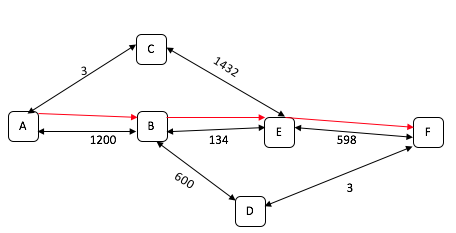
\includegraphics[width=8cm, height=6cm]{fig30}
		\caption{}
		\label{fig:ra1}
        \end{subfigure}%
	\hspace{30mm}
	\begin{subfigure}{0.32\textwidth}
        	\centering
		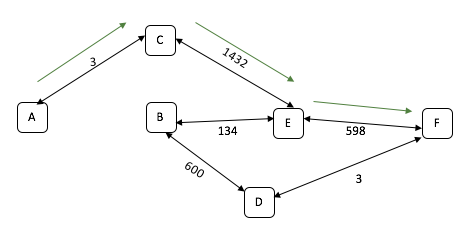
\includegraphics[width=8cm, height=6cm, clip,]{fig31}
		\caption{}
		\label{fig:ra2}
        \end{subfigure}
	\vfill
	\begin{subfigure}{0.32\textwidth}
        	\centering
		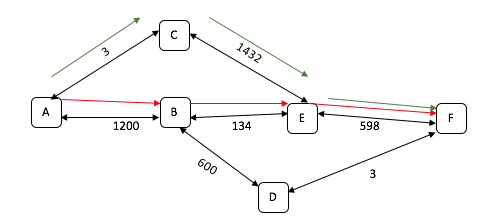
\includegraphics[width=8cm, height=6cm, clip]{fig32}
		\caption{}
		\label{fig:ra3}
        \end{subfigure}
\caption{Risk-aware Iterative partially disjoint shortest path (a) Find the shortest path in the network
(b) Remove the links as specified in the section 6.1.1 and run the Djikstra again (c)Add both the paths back on}
\label{fig:riskAwareAlgo}
\end{figure*}

%Fig. 6.1 Risk aware link Risk aware PDID disjoint


\subsection {Effects of Risk PDID link pruning} 
The expected increase in the failure with this approach is not just due to the partially disjoint paths. Risk aware PDID approach can only ignore the vulnerable path in the primary link and there is no guarantee that such a link would not exist in the backup path. In the figure 6.1, the backup path still has one of the links greater than 1000 km. But this scenario is common in the other algorithms as well. That said, Risk aware PDID still cuts down the probability of failure of a connection due to long distance links in to half just like the other two. 

\section {Performance analysis of Risk aware PDID}

\subsection {Blocking Probability}

%Fig. 6.2 Blocking of Risk aware PDID
\begin{figure}[hbt!]
\centering
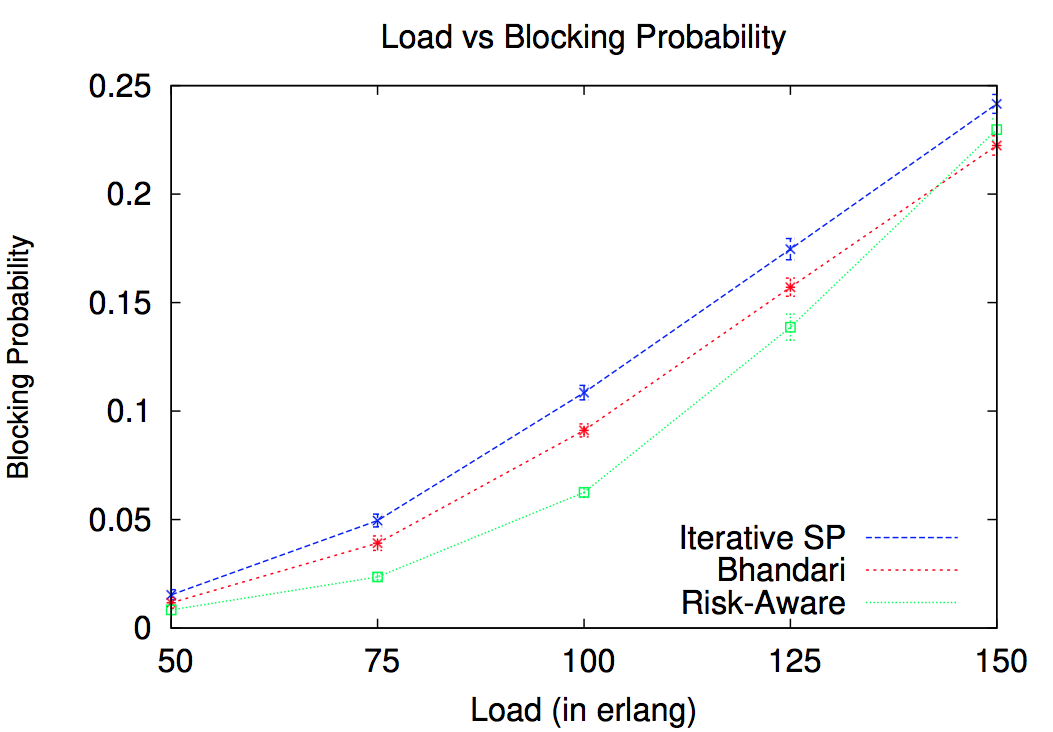
\includegraphics[width=12cm, height=8cm]{fig33.png}
\caption{Comparative analysis of Iterative shortest path, Bhandari shortest path and Risk aware PDID for blocking}
\label{fig:all3Block}
\end{figure}

	Unsurprisingly, the blocking probability is decreased for Risk aware PDID compared to Iterative Djikstra. But the plot seems to suggest some interesting facts between Risk aware PDID and Bhandari. At lower loads, Risk aware PDID shows better performance than Bhandari. Although this decrease is very small in the beginning, it increases with the increase in the load. At moderate load, Risk aware PDID shows at most 3\% decrease in blocking. This indicates that there are enough links still available for Risk aware PDID to allocate resources greedily for the connection and continues to outperform Bhandari. However, this does not last longer as further increase in load contributes to closing this gap between Bhandari and Risk aware PDID. At higher load, Bhandari still recovers as Risk aware PDID pays price for being greedy just like iterative Djikstra. 

\subsection {Failure}

% Failure Probability
\begin{figure}[hbt!]
\centering
\includegraphics[width=12cm, height=8cm, page=18]{fig34.png}
\caption{Comparative analysis of Iterative shortest path, Bhandari shortest path & Risk aware IPDSP for failure}
\label{fig:all3Fail}
\end{figure}

	As expected, the failure for Risk aware PDID dominates both Iterative Djikstra and Bhandari. The primary reason being disjoint, the probability that a failure of medium or small distance links would lead to connection failures as well. Moreover, removing the long distance links in the primary path may lead to longer backup path and hence makes it prone to failures. That said, the increase in failure is just 0.08 \% while it can offer 3 \% decrease in blocking.

	     
\section {Releasing the resources of failed path(s)}

For all the simulation results obtained above, the failed paths remain in the network blocking new connections. Revoking the bandwidth of failed path(s) make a way for new connections. You may see the drop in the blocking. 

%Fig. 6.4 Reduced blocking as a result of released resources
\begin{figure}[hbt!]
\centering
\includegraphics[width=12cm, height=8cm, page=18]{fig35.png}
\caption{Comparative analysis of Iterative Shortest path, Bhandari shortest path & Risk aware PDID for blocking after releasing resources of failed connections}
\label{fig:all3ReleaseBlock}
\end{figure}


 As you can see, the Iterative Djikstra with release of resources shows similar blocking characteristic with Bhandari without release. This is an indication of how poor iterative Djikstra performs for blocking. At the same time, risk-aware Risk aware PDID without release performs much better than Bhandari with release at low loads but cuts very earlier at moderate loads. Likewise, risk-aware with release does not seem to cut Bhandari with release because it's still operating at lower loads as a result of releasing the resources of failed connections. Thus, by releasing the resources you can prolong the benefits of risk-aware Risk aware PDID.
	
